%\documentclass[a4paper]{article}
%\usepackage[english,ukrainian]{babel}
%\usepackage[utf8x]{inputenc}
%\usepackage[a4paper,top=3cm,bottom=2cm,left=3cm,right=3cm,marginparwidth=1.75cm]{geometry}
%\usepackage{amsmath}
%\usepackage{graphicx}
%\usepackage[colorinlistoftodos]{todonotes}
%\title{}
%\author{Столова Олеся}

%\begin{document}
%\maketitle
\section{Протоколи розділення секретів}
\begin{flushright}
\emph{(Автор: Олеся Столова. Не редагувалось)}
\par \emph{(Версія від 20 січня 2017 р.)}
\end{flushright}

$A_i$, $i=\overline{1,n}$-учасники протоколу, $A_p$-арбітр
\\
\textbf{Задача 1. }$A_p$ має деякий секрет $S$  і цей секрет $S$ "розділяє" між учасниками $A_i$, $i=\overline{1,n}$ так, що кожен з них не знає ніякої інформації про секрет $S$, будь-які $k<n$ учасників про секрет $S$ також ніякої інформації не можуть отримати, а усі учасники $A_i$, $i=\overline{1,n}$ разом, повністю відновлюють $S$.
\\
\textbf{Задача 2.} $A_p$ секрет $S$ "розділяє" між учасниками $A_i$, $i=\overline{1,n}$ так, що будь-які $1\leq\ k<n$, секрет $S$ відновлюють повністю, а будь-які $r<k$ учасників про секрет $S$ ніякої інформації не отримають.

Вирішення цих задач криптографічними методами:
\begin{center}
\textbf{Протокол розділення секретів 1}
\end{center}
Задача 1. Арбітр $A_p$ має секрет $S=S_1,S_2,\ldots,S_t$, $S_i\in{\{0,1}\}$- випадкова послідовність.
Розділення секретів арбітром $A_p$
\begin{enumerate}
\item Генерується $n-1$ випадкова послідовніть з незалежними та рівноймовірними бітами, які не залежать також від $S=S_1,S_2,\ldots,S_t$.
\item Арбітр учаснику $A_i$ передає послідовність $S^{(i)}$, $i=\overline{1,n-1}$, а учаснику $A_n$ передає послідовність $S^{(n)}=S\oplus\oplus_{i=1}^n\ S^{(i)}$.
\end{enumerate}
Відновлення секрету $S$
Учасники $A_i$, $i=\overline{1,n}$ разом відновлюють секрет по формулі 
$s=\oplus_{i=1}^n\ S^{(i)}$.
Дійсно, $\oplus_{i=1}^n\ S^{(i)} =\oplus_{i=1}^{n-1}\ S^{(i)}\oplus\ S^{(n)}=\oplus_{i=1}^{n-1}\ S^{(i)}\oplus\ S\oplus\sum\limits_{i=1}^{n-1}\ S^{(i)}=S$.

Чому про $S$ менш ніж $n$ учасників нічого не дізнається?\\
а) Будь-які учасники з перших $n-1$ вочевидь про $S$ нічого не дізнаються.\\
б) Нехай в групі $r<n$ учасників присутні $A^{i}$, $i=\overline{1,r}$, $r<n-1$.\\
Нехай учасники складуть послідовність: $\oplus_{i=1}^r\ S^{(i)}\oplus\ S^{(n)}=S\oplus\sum\limits_{i=1}^{n-1}\ S^{(i)}\oplus\sum\limits_{i=1}^{r}\ S^{(i)}=S\oplus\oplus_{i=r+1}^{n-1}\ S^{(i)}$ (1) (Аналогія шифру Вернона) звідси дізнатися про $S$ якусь інформацію-неможливо.
\begin{center}
\textbf{Протокол розділення секретів 2}
\end{center}
$A_p$ має секрет $S\in(N)$
Розділення секрету $A_p$
\begin{enumerate}
\item Обираємо велике просте $p$, $p>s$ ($p$-відкрита інформація).
\item Обираємо $k-1$ випадкових елементів поля $F_p$: $a_i\in{\{1,...,p-1}\}$, $i=\overline{1,k-1}$ та вважають  $a_0=s$ будуємо поліном над $F_p$.
$f(x)=\sum\limits_{i=0}^{k-1}\ a_i x^{i}$ степені $k-1$, $a_{k-1}\ne 0$. Числа $a_i$ $i=\overline{1,k-1}$ та поліном - це секрет арбітра $A_p$
\item Кожному учаснику $A_i$ арбітр $A_p$  передає число $f(i)$, $i=\overline{1,n}$- номер учасника.Таким чином кожен учасник має пару $(i,f(i))$, $i=\overline{1,n}$.
\end{enumerate}

Відновлення секрету $S$

Нехай зібралися $k$ учасників $A_{i_l}$, $l=\overline{1,n}$.
Приклад: з поліномів $f:R\rightarrow R$

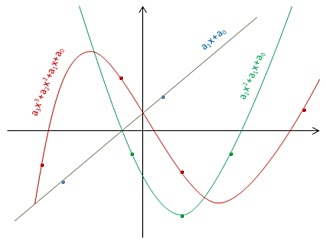
\includegraphics{PICTURE.jpg}
\\
$a_1 x+a_0$ - відновлюється по 2 точкам;
\\
$a_2x^2+a_1x+a_0$ - відновлюється по 3 точкам;
\\
$a_3x^3+a_2x^2+a_1x+a_0$- відновлюється по 4 точкам.

Розглянемо поліном 2ї степені:
складемо систему:
\begin{equation*}
 \begin{cases}
  a_2 x_1 ^2+a_1 x_1+a_0=y_1, 
   \\
  a_2x_2 ^2+a_1 x_2+a_0=y_2,
   \\
  a_2x_3 ^2+a_1 x_3+a_0=y_3.
 \end{cases}
\end{equation*}

\begin{enumerate}
\item Учасники $A_{i_l}$, $l=\overline{1,k}$ відновлюють поліном $f(x)$ по парам(по $k$ точкам):
${\{i_l, f(i_l),l=\overline{1,k}}\} $ за допомогою ітераційної формули Лагранжа $f(x)=\sum\limits_{l=1}^{k}\ f(i_l)\prod\limits_{j\ne l} {{x-i_j}\over{i_l-i_j}}$.
\item  Обчислюють $f(0)=a_0=s$.
\end{enumerate}
Чому число учасників $r<k$  про секрет $S$ не дізнаються ніякої інформації?\\
Нехай зібрались учасники $A_{i_l}$, $l=\overline{1,k-1}$. Вони мають $k-1$ пару ${\{i_l, f(i_l),l=\overline{1,k-1}}\} $.  (2)\\
Додамо до множини (2) пару $(0,U_k)$. Тоді через точки  ${\{(i_l,f(i_l)), i=\overline{1,k-1}, (0,U_k)}\} $, $U_k\in{F_p}$ можна побудувати поліном $\tilde{f}(x)$ степені $k-1$  та у цього поліному $f(0)=U_k$.

%\end{document}